\section{More tweezers per engine and per row}\label{sec:moretweezers}

This section asks how many independent tweezers one engine can carry, what limits the number, and how a stack
of engines can serve more sites than it has tweezers. The packing results are simulated on the
beam-propagation matrix of design D1, the star-coupler aberration with exact path lengths, and the transport
depths with a 1D classical Monte Carlo; the scaling tables are derived from these
(\texttt{docs/scaling.md}, \texttt{docs/scaling\_beyond.md}).

The answer in brief: the useful number of tweezers per row is the row length divided by the site pitch, and
the row length is set by the diffraction-limited field of the objective. A 192-port chip filling the
$\pm100$~\textmu m field of the proposal carries 45 tweezers on the 4~\textmu m site lattice and needs 383 fast
actuators. Sixteen such chips in the stacked relay of Sec.~\ref{sec:rows} give 720 simultaneous tweezers, and a
row-select tilt lets this one stack serve all 50 rows of the field, 2,250 sites, in four passes. The
per-tweezer costs, 8.7 fast actuators and about 57~mW at 1.2~mK, do not fall with scale. For comparison, the
1,024-atom assembly with crossed acousto-optic deflectors cited in the proposal moved a median of 13 (maximum 38)
atoms in parallel \cite{proposal}.

\subsection{Packing within a row}\label{sec:moretweezers-packing}

We filled the $\pm60$~\textmu m row of D1 with tweezers at spacing $s$, neighbours in phase quadrature, and
synthesised the port amplitudes by least squares. Table~\ref{tab:more-packing} and
Fig.~\ref{fig:more-packing} give the result. The peak per tweezer per unit port power stays at 0.256 from 6
to 2.5~\textmu m spacing, so the power per tweezer is independent of how many are lit. At 3~\textmu m the
barrier between neighbours is 78\% of the trap depth, which keeps the atoms separate; at 2.5~\textmu m the
independence degrades to the 1\% level, and at 2~\textmu m the spots merge. We take 3~\textmu m (2.8
resolution cells, or 1.75 spot widths) as the practical packing limit. It is set by the spot width
(1.71~\textmu m FWHM), hence by the NA: at fixed NA, a narrower spot needs a less apodised window, which raises
the tails.

\begin{table}[htbp]\centering\small
\caption{Packing a $\pm60$~\textmu m row of design D1 (beam-propagation matrix, least-squares synthesis,
neighbours in phase quadrature). Simulated.}
\label{tab:more-packing}
\begin{tabular}{ccccc}
\toprule
spacing & tweezers & intensity midway & others' change when & residual after \\
 & & between neighbours & one moves 0.25~\textmu m & switch-off \\
\midrule
6~\textmu m & 21 & $5\times10^{-4}$ & 0.11\%, 1.6~nm & $<10^{-5}$ \\
4~\textmu m & 31 & 3.8\% & 0.10\%, 2.6~nm & $10^{-5}$ \\
3~\textmu m & 41 & 22\% & 0.11\%, 3.3~nm & $9\times10^{-4}$ \\
2.5~\textmu m & 49 & 43\% & 0.79\%, 10~nm & $9\times10^{-3}$ \\
2~\textmu m & 61 & 76\% (spots merge) & 5.2\%, 74~nm & $7\times10^{-2}$ \\
\bottomrule
\end{tabular}
\end{table}

\begin{figure}[htbp]\centering
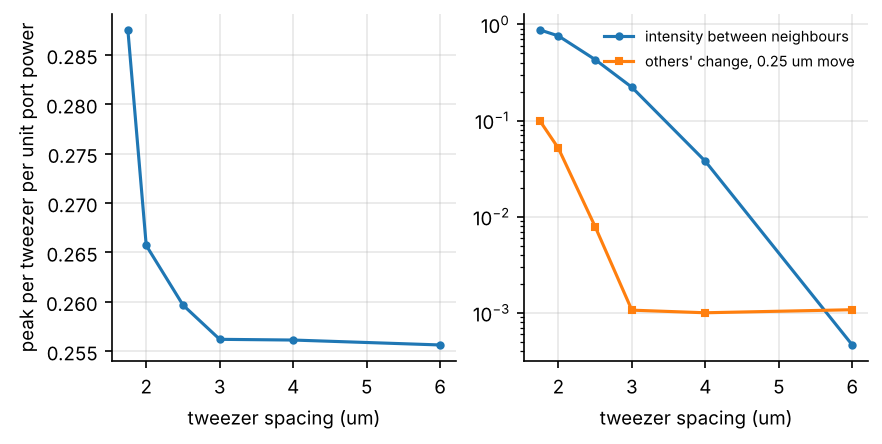
\includegraphics[width=0.85\linewidth]{m12_packing.png}
\caption{Packing limit of one engine, simulated on the beam-propagation response matrix of design D1 (128
ports, NA~0.5, 1064.4~nm) with least-squares synthesis of a $\pm60$~\textmu m row. Left: peak intensity per
tweezer per unit port power against tweezer spacing; it is flat at 0.256 from 6 to 3~\textmu m and rises only
as the spots merge. Right: intensity midway between neighbours (relative to the peak) and the largest change
of the other tweezers' depth when one tweezer moves by 0.25~\textmu m. Below 3~\textmu m the independence
degrades rapidly.}
\label{fig:more-packing}
\end{figure}

However, the proposal places atoms on a 4~\textmu m site lattice. The 41 tweezers of D1 at 3~\textmu m spacing
then reduce to 30 useful ones over the same $\pm60$~\textmu m. In general a row of length $L$ holds $L/4+1$
tweezers on 4~\textmu m sites, so the number per row cannot be raised by packing more densely. Scaling
therefore means longer rows and more rows.

\subsection{Ports per engine: field, actuators, power and slab}\label{sec:moretweezers-ports}

Each input port adds one resolution cell (1.06~\textmu m at NA~0.5) to the row. A row of $L$ thus needs $L/1.06$
ports, which is 3.8 ports and 7.5 to 8.7 fast actuators per tweezer, independent of $L$.
Table~\ref{tab:more-scaling} scales the engine with 1.5$\times$ oversampled arms, 2.0~\textmu m slab pitch and
1.5~\textmu m emitter pitch. The binding limits, in order, are (i) the objective field, (ii) the number, speed
and accuracy of the fast actuators, (iii) the laser power through each chip and (iv) the slab size. The
star-coupler aberration is not a limit below about 512 ports.

\begin{table}[htbp]\centering\small
\caption{Scaling of one focal-plane engine (1.5$\times$ oversampled arms, 2.0~\textmu m slab pitch,
1.5~\textmu m emitter pitch; row field 88\% of the port field). Fast actuators: two per port; data rate at
200~kHz and 16 bit. Aberration: worst-port rms arm-phase error on the Rowland circle (geometric lower bound).
Derived from the simulated packing and aberration results.}
\label{tab:more-scaling}
\begin{tabular}{cccccccc}
\toprule
ports & row field & tweezers at & slab radius & fast & static & data rate & aberration \\
 & & 4 / 3~\textmu m & / area & actuators & trims & & (rms) \\
\midrule
128 & 136~\textmu m & 30 / 40 & 1.3~mm / 0.5~mm$^2$ & 255 & 192 & 0.8~Gbit/s & 0.03~rad \\
\textbf{192} & \textbf{204~\textmu m} & \textbf{45 / 60} & \textbf{2.0~mm / 1.1~mm$^2$} & \textbf{383} & \textbf{288} & \textbf{1.2~Gbit/s} & \textbf{0.05~rad} \\
256 & 272~\textmu m & 60 / 80 & 2.7~mm / 2.0~mm$^2$ & 511 & 384 & 1.6~Gbit/s & 0.07~rad \\
512 & 545~\textmu m & 120 / 160 & 5.3~mm / 8.2~mm$^2$ & 1023 & 768 & 3.3~Gbit/s & 0.13~rad \\
1024 & 1090~\textmu m & 240 / 320 & 10.6~mm / 33~mm$^2$ & 2047 & 1536 & 6.6~Gbit/s & 0.27~rad \\
\bottomrule
\end{tabular}
\end{table}

\paragraph{Objective field.} The row can only be as long as the objective's diffraction-limited field. The
$\pm100$~\textmu m meta-objective target of the proposal corresponds to about 192 ports. Longer rows need a
larger corrected field at NA~0.5, which is the hardest optical requirement in the system. Refractive plan
objectives of NA~0.5 have flat fields of several hundred micrometres (recalled, to be verified). With a
$\pm250$~\textmu m field, 480 ports would give 110 tweezers per row, at a slab radius of about 5~mm and an
aberration of about 0.12~rad. A larger corrected field is the only route to longer rows.

\paragraph{Fast actuators.} Two per port: 383 for a 192-port row, each updated at $\ge200$~kHz (the
transport-heating limit at 1.2~mK) and accurate to about 1\% in amplitude and 10~mrad in phase for 10~nm
position noise. Beyond a few hundred channels per chip this needs drivers flip-chip bonded or co-integrated
with the photonics, and closed-loop calibration (on-chip power taps or camera feedback) against PZT hysteresis
and drift. This is the main engineering limit.

\paragraph{Power.} Power is linear in the number of simultaneous tweezers and in the depth. The engine design
gave 43~mW per 1.2~mK tweezer; the cross axis and the emitter facet loss raise this to 57~mW with the glued
collimator (factor 1.34, Sec.~\ref{sec:rows-collimator}). A full 192-port row of 45 tweezers then needs 2.6~W at
1.2~mK. An earlier plan to feed a row through 2 to 3 fibres into separate sub-trees is superseded: one
HI1060-matched input fibre per chip carries this power below the facet intensity cap
(Sec.~\ref{sec:rows-power}).

\paragraph{Slab and aberration.} The slab radius grows linearly with the port count (2~mm at 192 ports, 5~mm at
512). This fits within one die but exceeds a single electron-beam writing field, so stitching errors must be
absorbed by the static trims, or the slab written by DUV lithography. With the arm envelope produced by the
synthesis, the worst-port residual phase error grows linearly with size, about $0.033~\mathrm{rad}\times(\text{ports}/128)$
on the Rowland circle (port arc of radius $R/2$, Fig.~\ref{fig:more-aberration}). A quartic correction of the
port curve gains nothing, so the remainder comes from the circular arm arc; an aspheric arm curve would be the
next step beyond about 512 ports. These geometric values are about half the beam-propagation figure for D1
(0.079~rad), so they are lower bounds. Even doubled, they keep the Strehl ratio above 0.93 up to 512 ports.

\begin{figure}[htbp]\centering
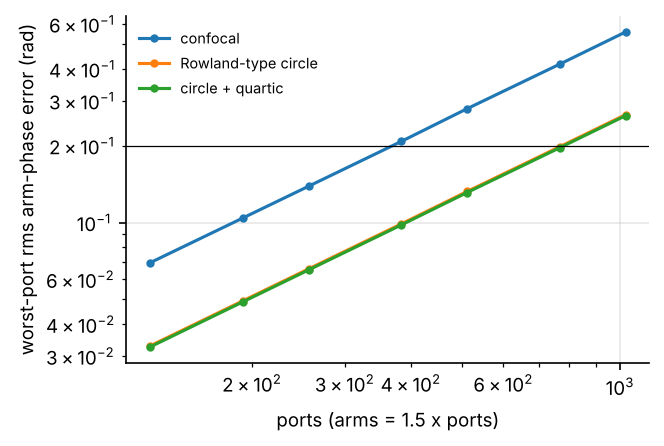
\includegraphics[width=0.65\linewidth]{m12_aberration.png}
\caption{Worst-port rms arm-phase error of the star coupler against the number of input ports (arms
$=1.5\times$ ports), computed from exact path lengths with the arm envelope of the least-squares synthesis, for
a confocal layout, a Rowland-type circle and a circle with quartic correction of the port curve. The
horizontal line marks 0.2~rad. The Rowland-type layout scales as about $0.033~\mathrm{rad}\times(\text{ports}/128)$;
the quartic correction adds nothing. Geometric values; the beam-propagation figure for D1 is about twice as
large.}
\label{fig:more-aberration}
\end{figure}

\paragraph{The 192-port chip.} We choose 192 ports because this matches the row to the $\pm100$~\textmu m field
of the proposal (a $\pm90$~\textmu m row on 4~\textmu m sites) and stays well inside the slab and aberration
limits (2.0~mm, 0.05~rad). It carries 45 tweezers on the site lattice (60 at the 3~\textmu m packing limit) with
383 fast actuators, 288 static trims and a data rate of 1.2~Gbit/s. The row length assumed here exceeds what
the adopted cylindrical collimator serves in the stacked relay: for D1, skew rays limit a row to
$|x_a|\le45$~\textmu m with the best common focus offset (Sec.~\ref{sec:rows-fill}). The counts below assume full
rows; Sec.~\ref{sec:combine} treats the skew-ray limit.

\subsection{Rows, stacks and row select}\label{sec:moretweezers-stack}

One engine addresses one row, and one chip with its collimator aligned to 0.1~\textmu m makes one row of the
stacked relay (Sec.~\ref{sec:rows}). We take 8 to 16 rows as the practical stack size; this is an engineering
judgement by analogy with laser-diode stacks, not a result. Sixteen chips make an 8~mm stack and 64~\textmu m of
rows, against a 200~\textmu m field.

\paragraph{Row select.} The pupil of the $y$ relay is conjugate to every chip's facet, and the atom plane to the
collimators' focal plane $S$. A tilt at any plane conjugate to the pupil therefore translates all rows of the
stack rigidly in $y$, without aberration in the paraxial limit. Shifting the 16 rows by 64~\textmu m is a
3.7~mrad tilt at the objective pupil. At the internal Fourier plane of the $y$ telescope, where the beam is 21.6
times smaller, it is 80~mrad optical, i.e.\ a 40~mrad mechanical rotation of a mirror about 1~mm tall in $y$
and about 20~mm wide. Placing rows to 10~nm needs about 6.5~\textmu rad of mechanical repeatability, which is
galvanometer-scanner class (recalled, to be verified against a specific scanner). Translating the whole stack
by 8~mm with 1~\textmu m accuracy is a slower alternative (1~\textmu m becomes 8~nm at the atoms). Atoms wait
in the static 1075~nm array between passes. A 16-chip stack then serves all 50 rows of the
$\pm100$~\textmu m field, 2,250 sites, in four passes, and the hardware per site drops by a factor 3.1. The same
tilt moves all rows of the stack together, so the stack can carry atoms in 2D: independently along $x$ within
each row, and in common along $y$. The scheduling of such passes is treated in Sec.~\ref{sec:rearrange}.

\paragraph{A second stack.} A polarising beam splitter before the objective combines a second 16-chip stack,
orthogonally polarised and offset by 64~\textmu m so the stacks never overlap. This doubles the simultaneous
capacity (32 rows, two passes) at twice the hardware, so the cost per tweezer is unchanged. It needs a
polarisation-insensitive objective, as does the polarisation option of Sec.~\ref{sec:rows-decorrelate}.
Table~\ref{tab:more-config} summarises the configurations.

\begin{table}[htbp]\centering\small
\caption{Configurations at 4~\textmu m site pitch (192-port chips except the first row; 57~mW per 1.2~mK
tweezer). Derived. Transport at lower depth reduces the power, see text.}
\label{tab:more-config}
\begin{tabular}{lcccccc}
\toprule
configuration & simultaneous & sites & passes & chips & fast & power at \\
 & tweezers & served & & & actuators & 1.2~mK \\
\midrule
one D1 chip (128 ports) & 30 & 30 & 1 & 1 & 255 & 1.7~W \\
one 192-port chip ($\pm90$~\textmu m row) & 45 & 45 & 1 & 1 & 383 & 2.6~W \\
stack of 16 & 720 & 720 & 1 & 16 & 6,128 & 41~W \\
\textbf{stack of 16 + row select} & \textbf{720} & \textbf{2,250} & \textbf{4} & \textbf{16} & \textbf{6,128} & \textbf{41~W} \\
two stacks (orthogonal pol.) + row select & 1,440 & 2,250 & 2 & 32 & 12,256 & 83~W \\
\bottomrule
\end{tabular}
\end{table}

\paragraph{Transport depth.} The 1.2~mK depth of the proposal is what fast long moves need: a 40~\textmu m move
in 100~\textmu s survives only at 1.2~mK even with a smooth trajectory, and with a 200~kHz staircase it does not
survive at any simulated depth, because each update step (up to 3.75~\textmu m) exceeds the 1.43~\textmu m
waist. Shorter or slower moves need much less depth. In a 1D classical Monte Carlo (4,000 atoms at
10~\textmu K, Gaussian potential with $w=1.43$~\textmu m, minimum-jerk trajectory, 200~kHz staircase), the
minimum depth for a loss $\le10^{-3}$ and an energy gain of at most one trap quantum per move is 0.2~mK for a
12~\textmu m (three-site) move in 200~\textmu s and 0.5~mK for a 40~\textmu m (ten-site) move in
200~\textmu s. For 12~\textmu m it is 0.8~mK at 100~\textmu s and 0.1~mK at 400~\textmu s; for 40~\textmu m no
depth up to 1.2~mK suffices at 100~\textmu s, and 0.2~mK does at 400~\textmu s. The excitation is
not monotonic in depth, because at some depths the trap frequency aliases with the update steps. This first
estimate cut the power of 720 tweezers from 41~W to 6.9 to 17~W. The 3D simulation with handoff to and from the
static array (Sec.~\ref{sec:transport}) has since revised it. The moving trap must be at least three times the
static hold depth, the hold about $20\,k_BT$, and moves must run along lanes between the rows. The minimum
moving depth is therefore 0.3~mK for 5~\textmu K atoms (0.6~mK for 10~\textmu K), not 0.2~mK, which gives 10
to 21~W for 720 tweezers (17 to 34~W for 1 to 2~\textmu K heating per move). Rearrangement mostly needs short
moves; a cycle of four passes at about 0.6~ms each (pick-up and release ramps assumed at 100~\textmu s each, a
200~\textmu s move and 200~\textmu s for the $y$ tilt to settle) takes 2 to 3~ms, and the depth can be raised for
the occasional long move.

\subsection{What does not work}\label{sec:moretweezers-not}

Three routes to more tweezers per chip fail. (i) Packing tweezers below the site pitch adds nothing on a
4~\textmu m lattice (Sec.~\ref{sec:moretweezers-packing}). (ii) Several emitter rows per chip cannot be
separated at the atoms: rows a few \textmu m apart on the facet land within nanometres of each other, and a separate collimator per emitter row cannot be fitted. (iii) Spectral
multiplexing of rows through the dispersive star coupler is excluded by the objective's chromatic focal shift
of 16~\textmu m/nm.

One untested route may remove the stack altogether: planar tiling of surface-emitting chips (speculative, not
simulated). Chips placed side by side on a common carrier, each with long grating emitters, would be imaged in
$y$ onto the atoms with demagnification $D$ = tile pitch/4~\textmu m, i.e.\ $D=1500$ for a 6~mm tile pitch. The
object-side NA in $y$ is then $3.3\times10^{-4}$, which a 2~mm weak grating radiates directly, so no collimator
is needed, and chip placement errors shrink by $D$ (10~\textmu m becomes 7~nm). The 0.1~\textmu m decentre
tolerance is replaced by an emission-angle tolerance of about 30~\textmu rad, i.e.\ $\delta n_\mathrm{eff}\sim3\times10^{-5}$,
trimmable with a heater (about 1.5~K) or by tilting the chip. The open questions are the grating efficiency
(emission up and down) and fitting the engine (slab of about 2~mm) and a 2~mm grating within one tile. Scaling
of these building blocks to $10^4$ to $10^6$ sites, with blocks of engines and the walls set by static
trapping power, the objective field and the 3~\textmu m lane distance, is the subject of
Sec.~\ref{sec:megascale}.
